\section{Network Performance Metrics}

When evaluating if a network is good or bad, there are two key metrics:
\emph{bandwidth} or \emph{throughput} and \emph{delay} or \emph{latency}.
A good network should have high bandwidth/throughput and low delay.

\subsection{Bandwidth and Throughput}
Bandwidth is the max number of bits that can sent through a network
per unit time, typically measured in bits per second (bps).
Bandwidth is a property of the physical network components. For instance,
a copper cable may have a bandwidth of 500 Mbps or a fiber optic cable
may have a bandwidth of 100 Gbps.


Throughput measures the bandwidth utilization of a network. It's also
measured in bits per second.
\begin{equation}
    0 \leq \text{throughput} \leq \text{bandwidth}
\end{equation}
Throughput is a function of the mechanisms used to communicate over the
physical network. Network throughput can be lower than network bandwidth
due to inefficiencies of communication mechanism, but a good network
will make throughput as high as possible.

\subsection{Latency}
Suppose you are sending a series of bits from point A to B. Delay or
latency is the total time between first bit leaving point A and last
bit reaching point B. It is measured in units of time, typically seconds
or milliseconds.
\marginnote{Internet for outer space is currently an area of research.
    Latency can be minutes, hours, or days in such a case. }
Note that, in a packet-switched network, the entire packet must be
received by the router. This "store-and-forward" model introduces
delays. An alternative with smaller delay is "cut-through", where
the router begins processing as soon as the destination address is
received. The tradeoff is that routers can't check for packet
corruption, since it necessarily requires the entire packet.

We represent delays with a timing diagram, as in Figure \ref{fig:timingdiagram}.

\begin{figure}
    \centering
    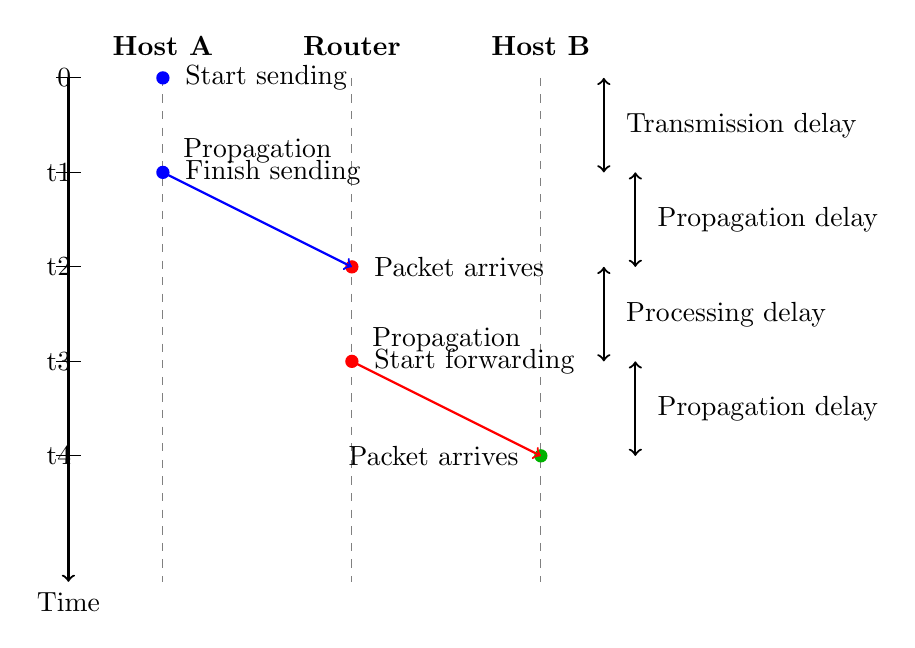
\begin{tikzpicture}[scale=0.8]
        % Time axis (vertical, going down)
        \draw[thick, ->] (-0.5, 0) -- (-0.5, -8) node[below] {Time};

        % Time labels
        \foreach \y/\label in {0/0, -1.5/t1, -3/t2, -4.5/t3, -6/t4} {
                \draw (-0.7, \y) -- (-0.3, \y) node[left] {\label};
            }

        % Host A, Router, Host B columns
        \node at (1, 0.5) {\textbf{Host A}};
        \node at (4, 0.5) {\textbf{Router}};
        \node at (7, 0.5) {\textbf{Host B}};

        % Vertical lines for each node
        \draw[dashed, gray] (1, 0) -- (1, -8);
        \draw[dashed, gray] (4, 0) -- (4, -8);
        \draw[dashed, gray] (7, 0) -- (7, -8);

        % Packet transmission events
        % Host A starts sending at t=0
        \fill[blue] (1, 0) circle (3pt);
        \node[right] at (1.2, 0) {Start sending};

        % Host A finishes sending at t₁
        \fill[blue] (1, -1.5) circle (3pt);
        \node[right] at (1.2, -1.5) {Finish sending};

        % Packet arrives at router at t₂
        \fill[red] (4, -3) circle (3pt);
        \node[right] at (4.2, -3) {Packet arrives};

        % Router starts forwarding at t₃
        \fill[red] (4, -4.5) circle (3pt);
        \node[right] at (4.2, -4.5) {Start forwarding};

        % Packet arrives at Host B at t₄
        \fill[green!70!black] (7, -6) circle (3pt);
        \node[left] at (6.8, -6) {Packet arrives};

        % Arrows showing packet flow
        \draw[->, thick, blue] (1, -1.5) -- (4, -3);
        \node[above, sloped] at (2.5, -1.5) {Propagation};

        \draw[->, thick, red] (4, -4.5) -- (7, -6);
        \node[above, sloped] at (5.5, -4.5) {Propagation};

        % Delay annotations
        \draw[<->, thick] (8, 0) -- (8, -1.5);
        \node[right] at (8.2, -0.75) {Transmission delay};

        \draw[<->, thick] (8.5, -1.5) -- (8.5, -3);
        \node[right] at (8.7, -2.25) {Propagation delay};

        \draw[<->, thick] (8, -3) -- (8, -4.5);
        \node[right] at (8.2, -3.75) {Processing delay};

        \draw[<->, thick] (8.5, -4.5) -- (8.5, -6);
        \node[right] at (8.7, -5.25) {Propagation delay};

    \end{tikzpicture}
    \caption{Timing Diagram}
    \label{fig:timingdiagram}
\end{figure}

There are different delays when packet routing:
\begin{itemize}
    \item Transmission Delay: Packet Size / Link Bandwidth
    \item Propagation Delay: Link Length / Link Propagation Speed
    \item Queuing Delay: Sum of Transmission Delay for all packets
          ahead in the queue
    \item Processing Delay: Depends upon the router hardware
          processing speed, nature of processing, etc.
\end{itemize}

The total delay for a single packet going over 2 hops in a
store-and-forward packet-switched network is
\begin{equation}
    2(TD + PD) + QD + PrD
\end{equation}

For $M$ hops ($M-1$ routers) the end-to-end delay is
\begin{equation}
    M (TD + PD) + (M - 1) (QD + PrD)
\end{equation}

For a store-and-forward model with $N$ packets over 1 hop,
the time from 1st bit leaving A to last bit of last packet
reaching B is
\begin{equation}
    N\times TD + PD
\end{equation}

For a store-and-forward model sending $N$ packets over $M$
hops, the total end-to-end delay is
\begin{equation}
    M \times (TD + PD) + (M-1) \times (QD + PrD) + (N-1) \times TD
\end{equation}

Queuing occurs at the router when the packet arrival rate
exceeds the packet drain rate.

